\documentclass[kulak]{kulakarticle} % options: kulak (default) or kul

\usepackage[dutch]{babel}
\usepackage{pdfpages}
\usepackage{graphicx}


\title{Smart Fire Extinguisher - Tussentijds Verslag}
\author{TEAM 6: Anna-Laura, Emile, Jérôme, Jesse}
\date{Academiejaar 2022 -- 2023}
\address{
	\textbf{Groep Wetenschap \& Technologie Kulak} \\
	Ingenieurswetenschappen \\
	P\&0 2}

\begin{document}

\maketitle

\section*{Inleiding}

Bij de brandbestrijding in grote warenhuizen worden momenteel sprinklers gebruikt. Deze zijn vastgemaakt aan het plafond van het gebouw en zijn aan de waterleiding aangesloten om bij brand water in alle richtingen te doen neerdalen en de brand te blussen. Het blussen van branden gaat dus heel goed met het gebruik van sprinklers, maar er zijn ook bepaalde nadelen aan. De aanleg en het onderhoud van alle leidingen die de sprinklers van water voorzien is een hele dure onderneming. Ook kan bij het springen van een van de waterleidingen heel veel water verloren gaan alsook goederen beschadigen. Ook bij het blussen van een brand kan het bestrijkingsgebied van het water groter zijn dan waar de brand zich bevind, hierdoor kunnen er meer goederen verloren gaan. \\

Daarom zijn wij op zoek gegaan naar een efficientere manier om branden te blussen. Een Smart Fire Extinguisher, die zelf de branden kan detecteren, localiseren en gericht kan blussen. Zo zou 1 apparaat (met dus maar 1 aansluiting op de waterleiding of een eigen waterreservoir) een groot oppervlakte brandveilig kunnen maken. Dit zou het veel goedkoper maken voor de eigenaar. Bovendien worden de branden veel gerichter geblust waardoor er minder kans is op waterschade.


\section{Ontwerp}

We opteren voor een stationair brandblusplatform dat gebruik maakt van twee armen om het water in de juiste richting en onder de juiste hoek weg te spuiten. Water uit een waterreservoir zal dan met behulp van een pomp op de gewenste plaats terecht komen. Deze plaats zal zijn vastgesteld door een camera. Deze detecteert de brand en aan de hand van de beelden zal er berekend worden waar en hoe ver de brand zich bevind ten opzichte van het brandblusplatform. Daarna zullen nog een hoop berekeningen de hoek van de twee armen bepalen. \\

Voor het detecteren van de brand maken we gebruik van een webcam (USB Webcam 1080P), in Python wordt een programma geschreven op een laptop die aan branddetectie en -localisatie doet. \\

De beweging van de armen gebeurt met behulp van twee motoren (Micro Metal Gear Motor 100:1 HP), deze zullen we met behulp van {\bf{--OFWEL voltage regulator OFWEL motor driver--nog te bekijken--}} met de gewenste snelheid en in de juiste richting doen draaien. Volgens de berekeningen gedaan door de webcam en een laptop kunnen de armen zich juist positioneren.

Als de armen juist staan, is het enige dat overblijft het blussen van de brand. Hiervoor zal de pomp (Membraanpomp 12V 4.8 bar) water uit het waterreservoir (jerrycan 10L) door een dunne slang pompen, om zo weggespoten te worden richting het doelwit. {\bf{Het water de juiste snelheid doen gaan om de maximale nodige afstand te halen zal gebeuren met behulp van een spuitstuk op het einde van de slang met een kleinere diameter.}}
\\
bla
\\
blq
\\
bla
\\

\section{Berekeningen}
\subsection{Water}

\begin{figure} [h!]
	\centering
	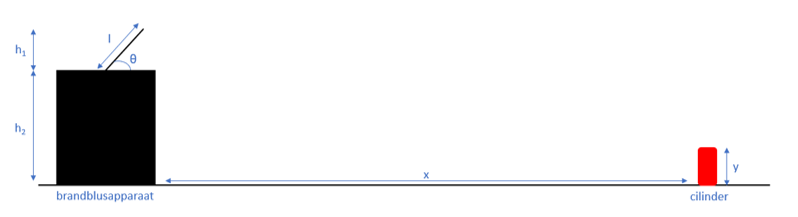
\includegraphics[width = 1 \textwidth]{schematische voorstelling water LATEX}
	\caption{Schematische voorstelling van de opstelling}
	\label{schematische voorstelling}
\end{figure}
De maximale afstand \(x\) zoals te zien in afbeelding \ref{schematische voorstelling} tussen het brandblusapparaat en de cilinder is \(10,45m\).
\subsection{Camera}
\begin{figure}
	\centering
	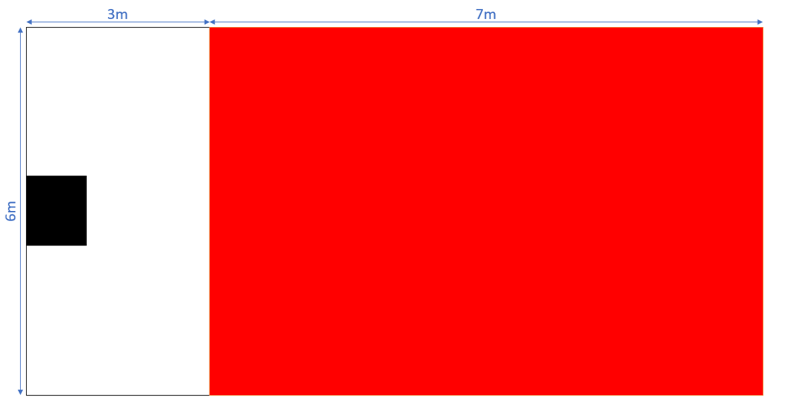
\includegraphics{schematische voorstelling bestrijkingsgebied LATEX}
	\caption{Schematische voorstelling van het bestrijkingsgebied}
	\label{bestrijkingsgebied}
\end{figure}


\subsection{Armen}



\section{Planning}
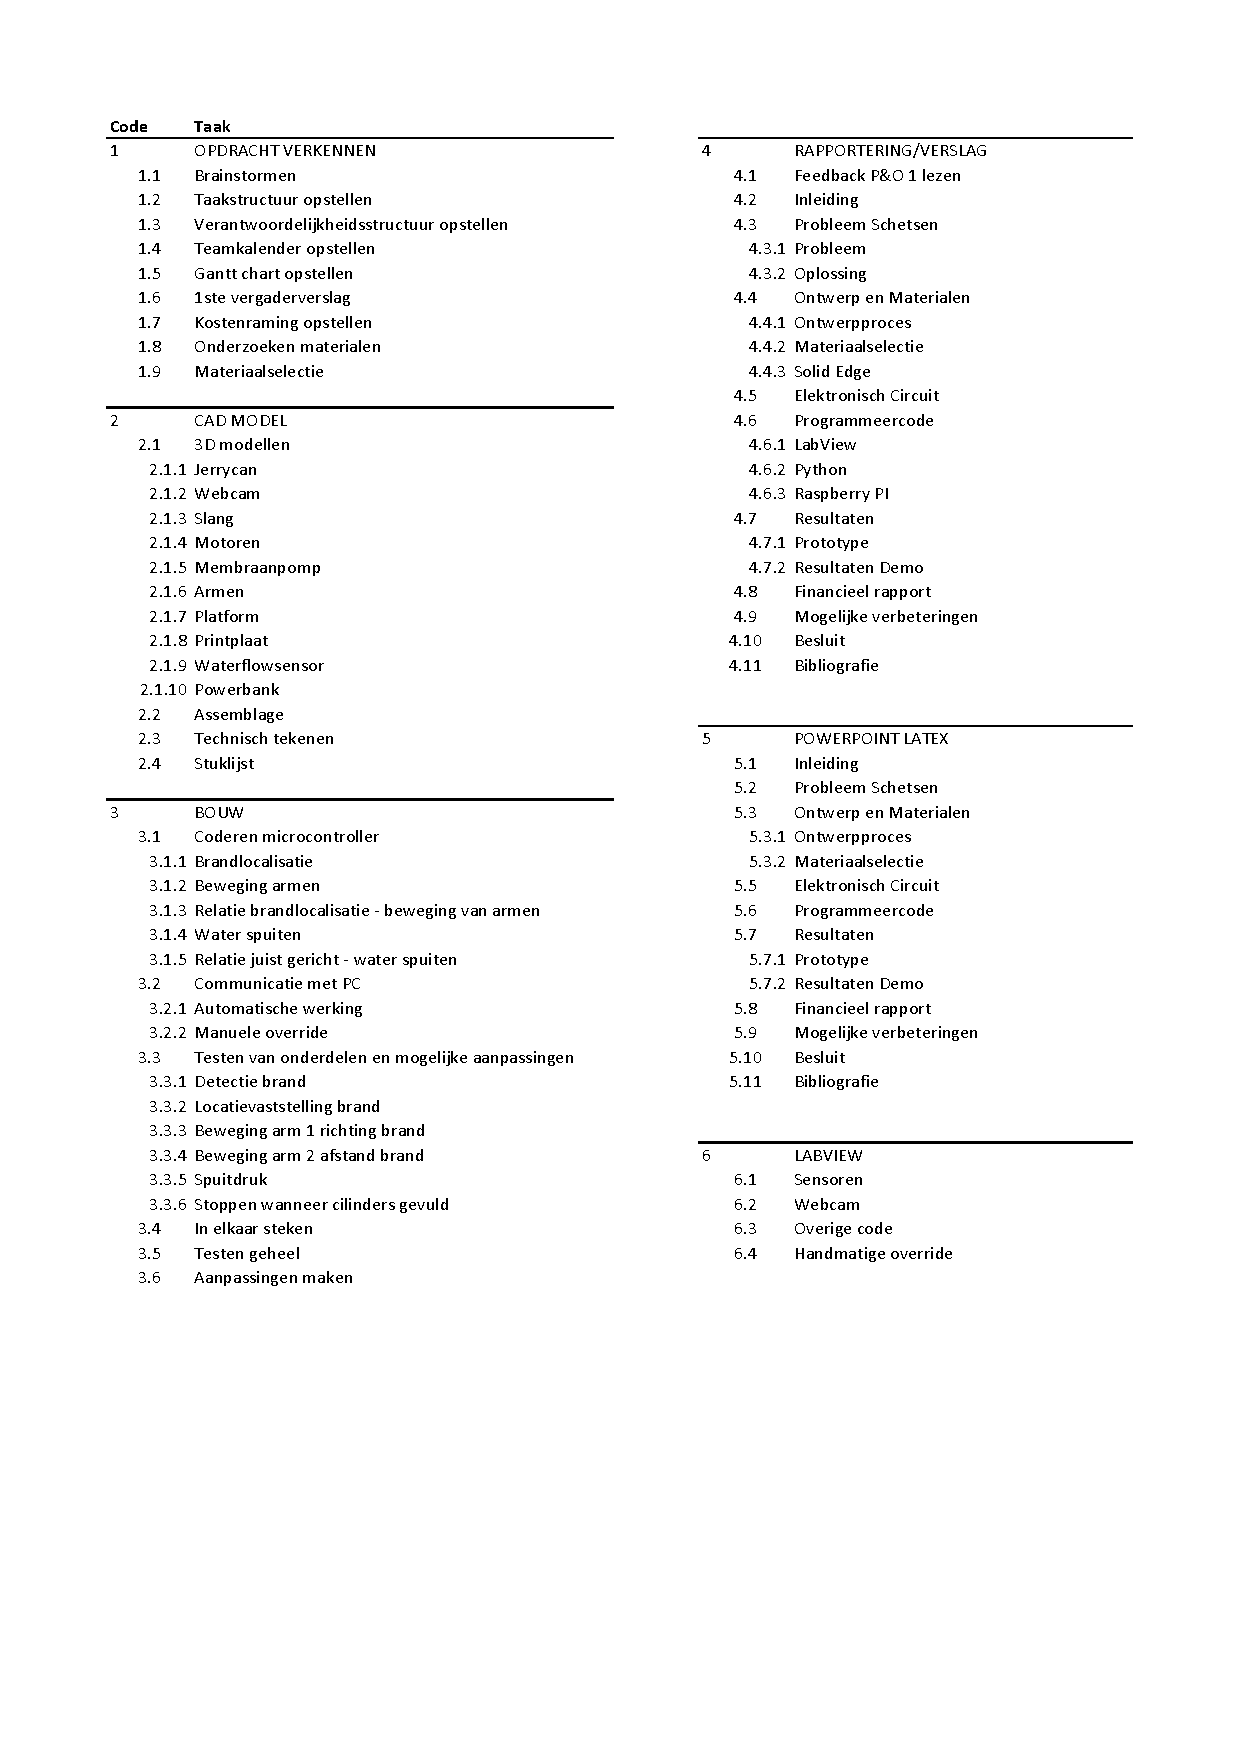
\includepdf{taakstructuur_LATEX_2.pdf}
\begin{figure} 
	\centering
	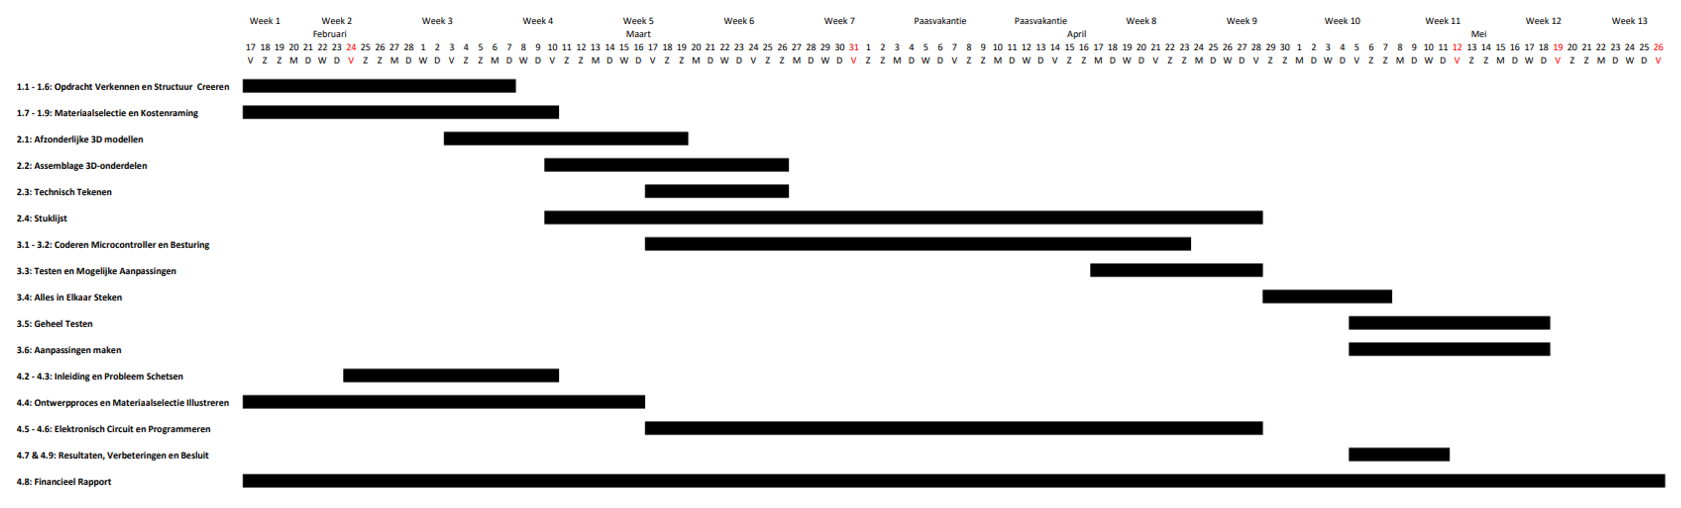
\includegraphics[width=1.45\textwidth, angle = 270 ]{ganttchart_LATEX}
\end{figure}


\section{Vooruitgang}


\section*{Besluit}

Afsluitende tekst.

\end{document}
